\documentclass[aspectratio=169,xcolor=table]{beamer}
%aspcetratio >> 1610 169 149 54 43 32
%The themes:
\usetheme[style=classic]{mharvellous}
%\usetheme[style=dark]{mharvellous}
%\usetheme[style=mracula]{mharvellous}
% \usetheme[style=default]{mharvellous}
%*--------------------------------------------------
%\usepackage{helvet}
%*--------------------------------------------------
\usepackage{bibunits}  
%\setbeamertemplate{bibliography item}{[\theenumiv]}
\setbeamertemplate{bibliography item}{\insertbiblabel}
\defaultbibliography{bibliography}
%\defaultbibliographystyle{IEEEtran}
%\defaultbibliographystyle{amsalpha}
\defaultbibliographystyle{abntex2-alf}
%\bibliography{bibliography}
%\usepackage[backend=biber,style=alphabetic,citestyle=authoryear]{biblatex}
% \addbibresource{bibliography.bib}
%\usepackage{natbib}
\usepackage{bibentry}
%*--------------------------------------------------
\usepackage{lipsum}
\usepackage{epigraph}
\usepackage{graphicx}
\usepackage{multirow}
%\usepackage{enumitem}
\usepackage{array}
%\usepackage{multimedia}
\usepackage{media9}
%\usepackage{pdfpc-movie}
\usepackage{circledsteps}
\usepackage{listings}
\usepackage[normalem]{ulem}
%\usepackage{Sweave}
%\usepackage{xkeyval}
%\usepackage{palatino}
%\usepackage{pgfpages}
\usepackage{float}
%*--------------------------------------------------
\usepackage[timeinterval=1]{tdclock}
%\usepackage[font=Times,timeinterval=1, timeduration=200,resetatpages=all]{tdclock}
%\usepackage[font=Times,timeinterval=10, timeduration=2.0, timedeath=0, fillcolorwarningsecond=white!60!yellow,timewarningfirst=50,timewarningsecond=80,resetatpages=2]{tdclock}
%*--------------------------------------------------
\usepackage{url}
\usepackage{tabularx,booktabs}
\usepackage{threeparttable}
\usepackage[absolute, overlay]{textpos}
%*--------------------------------------------------
\usepackage{framed, color}
\usepackage[tikz]{bclogo}
\usepackage{spot}
\setspotlightcolor{red!50}
% %\setspotlightstyle{star, fill=red!50}
% %\setspotlightstyle{star points=7}
\usepackage{color,soul}
%\usepackage{xcolor}
\usepackage{tcolorbox}
\usepackage{xcolor}
\usepackage[export]{adjustbox}
\usepackage{verbatim}
\usetikzlibrary{trees,shapes,arrows}
\usepackage{fancyvrb}
\usepackage{float}
%*--------------------------------------------------
\usepackage{amsmath}
\usepackage{xfrac}
\usepackage{units}
\usepackage{ulem}
%*-------------------------------------------------------------------------------
%\newcolumntype{C}[1]{>{\centering\arraybackslash}m{#1}}
\newcolumntype{L}[1]{>{\raggedright\let\newline\\\arraybackslash\hspace{0pt}}m{#1}}
\newcolumntype{C}[1]{>{\centering\let\newline\\\arraybackslash\hspace{0pt}}m{#1}}
\newcolumntype{R}[1]{>{\raggedleft\let\newline\\\arraybackslash\hspace{0pt}}m{#1}}
%*-------------------------------------------------------------------------------
%\pgfpagesuselayout{2 on 1}[a4paper,border shrink=5mm]
%\setbeamertemplate{note page}[plain]
%\setbeameroption{show notes on second screen=bottom}
%*-------------------------------------------------------------------------------
\setbeameroption{hide notes}
%\setbeameroption{show only notes}
%\setbeameroption{show notes on second screen=right}
\setbeamertemplate{note page}{\pagecolor{yellow!5}\insertnote}
%*-------------------------------------------------------------------------------

%*-------------------------------------------------------------------------------
\title              {Revisão de Álgebra}
\subtitle           {Parte 1 - Geometria Analítica e Álgebra Linear}
\author             {Juliana Santana}
\email              {juliana.maria@fbter.org.br}
\advisor            {Orientador: Marco A. dos Reis}
\institute          {Robótica e Sistemas Autônomos, Senai Cimatec}
\date               {Maio de 2022}
% \ulogo        		{Template/logosenaicimatecnegativo}
% \ulogof             {Template/logosenaicimatec2020}
% \ulogoo        		{Template/rosa-logo}
% \ulistelement    	{Template/bullet-white}

%*-------------------------------------------------------------------------------
\graphicspath{{Source/pictures/}}
%*-------------------------------------------------------------------------------
\totalNoSlidesDisabled % To turn off the total number of slides in the footer. Comment this if you want the total number of slides in the footer
%*-------------------------------------------------------------------------------
\begin{document}
%*----------- COVER -------------------------------------------------------------
 \begin{frame}[t,plain]
%*----------- sound--------------------------------
    \includemedia[
        %width=1ex,
        %height=1ex,
        %activate=pageopen, 
        activate=onclick,
        deactivate=onclick,
        %passcontext,
        transparent,
        addresource=./Source/sounds/hip-hop.mp3,
        flashvars={
                    source=./Source/sounds/hip-hop.mp3
                    %&autoPlay=true
                    &autoRewind=true
                    &Play=2s
                    &repeat=always
                    %&Loop=true
        }
    ]
    {}{VPlayer.swf}
%*----------- start-page--------------------------
    \titlepage
    %*----------- notes-------------------------------
    \note[item]{Notes can help you to remember important information. Turn on the notes option.}
\end{frame}
%-
%*----------- SECTIONS ----------------------------------------------------------
%*----------- SLIDE -------------------------------------------------------------
\begin{frame}[t]{A Álgebra Linear} 

 É uma área da matemática que que permite estudos matemáticos mais aprofundados e soluções em aplicações práticas em diversos campos da ciência e negócios.
 \nocite{baldin2011geometria}\nocite{boldrini1980algebra}\nocite{craig2012robotica}

 \vspace*{0.8cm}

\begin{figure}
    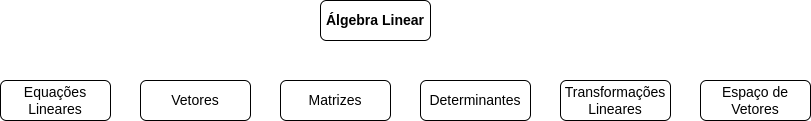
\includegraphics[width=\textwidth]{intro2.png}
\end{figure}
            
    \note[item]{Notes can help you to remember important information. Turn on the notes option.}
\end{frame}
%-

%*----------- SLIDE -------------------------------------------------------------
\begin{frame}[t]{Matriz e Vetores} 
    \begin{columns}
        \column{.01\textwidth}
        \column{.50\textwidth}
        \begin{itemize}
            \item Permitem escrever sistemas lineares de uma forma mais compacta
            \item E, utilizar operações com as matrizes para solucionar o sistema.
        \end{itemize}
        \column{.5\textwidth}
        \begin{figure}
            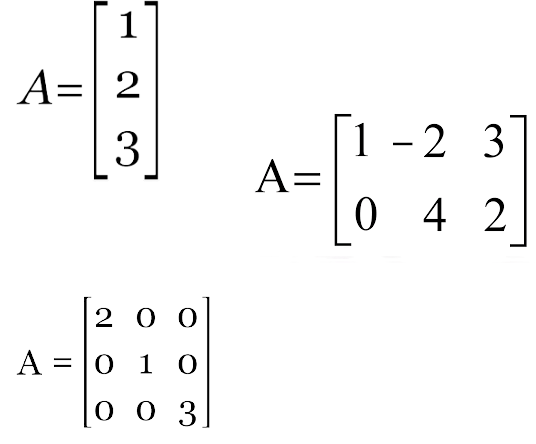
\includegraphics[width=0.8\textwidth]{matriz.png}
        \end{figure}
    \end{columns}
%*----------- notes
    \note[item]{Notes can help you to remember important information. Turn on the notes option.}
\end{frame}
%-
%*----------- SLIDE -------------------------------------------------------------
\begin{frame}[t]{Operações básicas com matrizes} 
    \framesubtitle{Soma e subtração}
 
    As \textbf{matrizes} devem ter a mesma dimensão. \\
    \vspace*{0.3cm}
    Operação de soma
    \begin{equation}
        \begin{pmatrix}
            1 & 2 \\
            3 & 4 \\
            5 & 6 \\
        \end{pmatrix}
        +
        \begin{pmatrix}
            6  & 5 \\
            4  & 3 \\
            2  & 1 \\
        \end{pmatrix}
        =
        \begin{pmatrix}
            1 + 6  & 2 + 5  \\
            3 + 4  & 4 + 3  \\
            5 + 2  & 6 + 1  \\
        \end{pmatrix}
        =
        \begin{pmatrix}
            7  & 7 \\
            7  & 7 \\
            7  & 7 
        \end{pmatrix}
    \end{equation}
    \vspace*{0.3cm}
    Operação de subtração
    \begin{equation}
        \begin{pmatrix}
            1 & 2 \\
            3 & 4 \\
            5 & 6 \\
        \end{pmatrix}
        -
        \begin{pmatrix}
            6  & 5 \\
            4  & 3 \\
            2 & 1 \\
        \end{pmatrix}
        =
        \begin{pmatrix}
            1 - 6  & 2 - 5  \\
            3 - 4  & 4 - 3  \\
            5 - 2  & 6 - 1  \\
        \end{pmatrix}
        =
        \begin{pmatrix}
           -5  & -3 \\
           -1  &  1 \\
            3  &  5 \\
        \end{pmatrix}
    \end{equation}
%*----------- notes
    \note[item]{Notes can help you to remember important information. Turn on the notes option.}
\end{frame}
%-

%*----------- SLIDE -------------------------------------------------------------
\begin{frame}[t]{Operações básicas com matrizes} 
    \framesubtitle{Multiplicação escalar}

    Operação de multiplicação por escalar

    \vspace*{0.8cm}

    \begin{equation}
        10
        *
        \begin{pmatrix}
            1 & 2 \\
            3 & 4 \\
            5 & 6 \\
        \end{pmatrix}
        =
        \begin{pmatrix}
            10 * 1  & 10 * 2  \\
            10 * 3  & 10 * 4  \\
            10 * 5  & 10 * 6  \\
        \end{pmatrix}
        =
        \begin{pmatrix}
            10  & 20 \\
            30  & 40\\
            50  & 60 
        \end{pmatrix}
    \end{equation}
    \vspace*{0.3cm}
%*----------- notes
    \note[item]{Notes can help you to remember important information. Turn on the notes option.}
\end{frame}
%-
%*----------- SLIDE -------------------------------------------------------------
\begin{frame}[t]{Operações básicas com matrizes} 
    \framesubtitle{Multiplicação}

    As \textbf{matrizes} só podem ser multiplicadas somente se o número de colunas no fator da esquerda é igual ao número de linhas no fator da direita. \\
    \begin{equation}
        m x \textcircled{n} * \textcircled{n} x p = m x p
    \end{equation}
    \vspace*{0.3cm}
    Operação de multiplicação entre matrizes
    \begin{equation}
        \begin{pmatrix}
            1 & 2 \\
            3 & 4 \\
            5 & 6 \\
        \end{pmatrix}
        *
        \begin{pmatrix}
            x_1 & y_1 \\
            x_2 & y_2 \\
        \end{pmatrix}
        =
        \begin{pmatrix}
            1x_1 + 2x_2  & 1y_1 + 2y_2  \\
            3x_1 + 4x_2  & 3y_1 + 4y_2  \\
            5x_1 + 6x_2  & 5y_1 + 6y_2  \\
        \end{pmatrix}
    \end{equation}
    \vspace*{0.3cm}
%*----------- notes
    \note[item]{Notes can help you to remember important information. Turn on the notes option.}
\end{frame}
%-
%*----------- SLIDE -------------------------------------------------------------
\begin{frame}[t]{Tipos de matrizes} 
    \framesubtitle{Matriz zero}
 
    A \textbf{matriz zero} possui todos os elementos iguais a zero.
    \vspace*{0.8cm}

    \begin{columns}[c]
        \column{.3\textwidth}
        \begin{equation}
            \begin{pmatrix}
                0 & 0 \\
                0 & 0 \\
            \end{pmatrix}
        \end{equation}
    
       \column{.35\textwidth}
       \begin{equation}
        \begin{pmatrix}
            0 \\
            0 \\
            0 \\
            0
            \end{pmatrix}
        \end{equation}

        \column{.35\textwidth}
        \begin{equation}
         \begin{pmatrix}
             0 & 0  & 0\\
             0 & 0  & 0\\

             \end{pmatrix}
         \end{equation}

   \end{columns}
    
%*----------- notes
    \note[item]{Notes can help you to remember important information. Turn on the notes option.}
\end{frame}
%-

%*----------- SLIDE -------------------------------------------------------------
\begin{frame}[t]{Tipos de matrizes} 
    \framesubtitle{Matriz transposta}

    A \textbf{matriz transposta} troca as linhas e as colunas em uma matriz.
    \begin{equation}
        \begin{bmatrix}
            1 & 3 & 5\\
            2 & 4 & 6\\
         \end{bmatrix}^\top =
            \begin{bmatrix}
            1 & 2 \\
            3 & 4 \\
            5 & 6   
         \end{bmatrix}
    \end{equation}
    \vspace*{0.3cm}
%*----------- notes
    \note[item]{Notes can help you to remember important information. Turn on the notes option.}
\end{frame}
%-
%*----------- SLIDE -------------------------------------------------------------
\begin{frame}[t]{Tipos de matrizes} 
    \framesubtitle{Matriz simétrica}

    A \textbf{matriz simétrica} é uma matriz que é simétrica em volta da sua diagonal principal. Por causa desta característica, a matriz simétrica é sempre igual a sua transposta. 
    \begin{equation}
            \begin{bmatrix}
            \textcolor{red}{1} & 5 & 6 & 7\\
            5 & \textcolor{red}{2} & 8 & 9\\
            6 & 8 & \textcolor{red}{3} & 10\\ 
            7 & 9 & 10 & \textcolor{red}{4}\\ 
         \end{bmatrix}
    \end{equation}
    \vspace*{0.3cm}
%*----------- notes
    \note[item]{Notes can help you to remember important information. Turn on the notes option.}
\end{frame}
%-
%*----------- SLIDE -------------------------------------------------------------
\begin{frame}[t]{Tipos de matrizes} 
    \framesubtitle{Matriz triangular superior e triangular inferior}

    A \textbf{matriz triangular} é uma matriz quadrada onde os elementos ou acima ou abaixo da diagonal principal são todos iguais a zero.
    \vspace*{0.8cm}


    \begin{columns}[c]
        \column{.5\textwidth}
        \centering
        Matriz triangular superior
        \begin{equation}
                \begin{bmatrix}
                \textcolor{red}{1} & 5 & 6 & 7\\
                0 & \textcolor{red}{2} & 8 & 9\\
                0 & 0 & \textcolor{red}{3} & 10\\ 
                0 & 0 & 0 & \textcolor{red}{4}\\ 
             \end{bmatrix}
        \end{equation}
    
       \column{.5\textwidth}
       \centering
       Matriz triangular inferior
       \begin{equation}
               \begin{bmatrix}
               \textcolor{red}{1} & 0 & 0 & 0\\
               5 & \textcolor{red}{2} & 0 & 0\\
               6 & 8 & \textcolor{red}{3} & 0\\ 
               7 & 9 & 10 & \textcolor{red}{4}\\ 
            \end{bmatrix}
       \end{equation}
   \end{columns}
%*----------- notes
    \note[item]{Notes can help you to remember important information. Turn on the notes option.}
\end{frame}
%-
%*----------- SLIDE -------------------------------------------------------------
\begin{frame}[t]{Tipos de matrizes} 
    \framesubtitle{Matriz diagonal}

    A \textbf{matriz diagonal} é uma matriz quadrada onde todos os elementos que não fazem parte da diagonal principal são iguais a zero.
    \vspace*{0.5cm}

    \begin{equation}
            \begin{bmatrix}
            \textcolor{red}{1} & 0 & 0 & 0\\
            0 & \textcolor{red}{2} & 0 & 0\\
            0 & 0 & \textcolor{red}{3} & 0\\ 
            0 & 0 & 0 & \textcolor{red}{4}\\ 
         \end{bmatrix}
    \end{equation}
%*----------- notes
    \note[item]{Notes can help you to remember important information. Turn on the notes option.}
\end{frame}
%-

%*----------- SLIDE -------------------------------------------------------------
\begin{frame}[t]{Tipos de matrizes} 
    \framesubtitle{Matriz identidade}

    A \textbf{matriz identidade} é uma matriz quadrada com \textit{n} linhas onde todos os elementos na diagonal principal são iguais a 1 e todos os outros elementos são 0.
    \vspace*{0.5cm}

    \begin{equation}
            \begin{bmatrix}
            \textcolor{red}{1} & 0 & 0 & 0\\
            0 & \textcolor{red}{1} & 0 & 0\\
            0 & 0 & \textcolor{red}{1} & 0\\ 
            0 & 0 & 0 & \textcolor{red}{1}\\ 
         \end{bmatrix}
    \end{equation}
%*----------- notes
    \note[item]{Notes can help you to remember important information. Turn on the notes option.}
\end{frame}
%-
%*----------- SLIDE -------------------------------------------------------------
\begin{frame}[t]{Tipos de matrizes} 
    \framesubtitle{Matriz inversa}

    Se o produto de duas \textbf{matrizes quadradas} é uma \textbf{matriz identidade}, então as duas matrizes são \textbf{inversas} uma da outra.


    \begin{equation}
        \begin{pmatrix}
            1 & 2 \\
            3 & 4 \\
        \end{pmatrix}
        *
        \begin{pmatrix}
            x_{11} & x_{12} \\
            x_{21} & x_{22} \\
        \end{pmatrix}
        =
        \begin{pmatrix}
            1 & 0 \\
            0 & 1 \\
        \end{pmatrix}
    \end{equation}
%*----------- notes
    \note[item]{Notes can help you to remember important information. Turn on the notes option.}
\end{frame}
%-
%*----------- SLIDE -------------------------------------------------------------
\begin{frame}[t]{Determinante} 

    O determinante permite verificar se uma matriz possui uma inversa ou não. Caso o determinante da matriz seja \textbf{diferente} de zero, a matriz possui uma inversa.

    \vspace*{0.3cm}

    \begin{equation}
        \det\begin{pmatrix}
            3 & 0 \\
            0 & 2 \\
        \end{pmatrix}
        =
        3*2-0*0
        =
        6
    \end{equation}

    \vspace*{0.3cm}

    \begin{columns}[c]
        \column{.4\textwidth}
        \hspace*{0.0cm}
        \centering
        O cálculo do determinante envolve a regra de \textbf{Sarrus}.
       \column{.6\textwidth}
       \centering
       \begin{figure}
        
\includegraphics[width=0.6\textwidth]{sarrus_rule.png}
    \end{figure}
   \end{columns}
%*----------- notes
    \note[item]{Notes can help you to remember important information. Turn on the notes option.}
\end{frame}
%-

%*----------- SLIDE -------------------------------------------------------------
\begin{frame}[t]{Sistemas de equações lineares} 

   Um dos problemas mais importantes na matemática é o da resolução de um \textbf{sistema de equações lineares}. 
   
   De acordo com \cite{leon2000algebra}, mais de 75\% de todos os problemas matemáticos encontrados em aplicações científicas e industriais envolvem a resolução de um sistema linear em algum estágio.

   \vspace*{0.45cm}

   \centering

   $a_{1}x+{1} + a_{2}x+{2} + a_{n}x+{n} = b$

   $a_{1}x+{1} + a_{2}x+{2} + a_{n}x+{n} = b$

   .

   .

   .

   $a_{1}x+{1} + a_{2}x+{2} + a_{n}x+{n} = b$

%*----------- notes
    \note[item]{Notes can help you to remember important information. Turn on the notes option.}
\end{frame}
%-
%*----------- SLIDE -------------------------------------------------------------
\begin{frame}[t]{Mínimos Quadrados} 

    O ajuste por mínimos quadrados é uma técnica de otimização matemática que busca \textbf{minimizar} a soma dos quadrados das diferenças entre o valor estimado e os dados observados.
 
    \vspace*{0.45cm}
 
\begin{columns}[c]
    \column{.5\textwidth}
    % \hspace*{0.9cm}
    \centering
    A técnica dos mínimos quadrados foi desenvolvida independentemente por \textbf{Adrien-Marie Legendre} e \textbf{Carl Friendrich Gauss}.
   \column{.5\textwidth}
   \centering
   \begin{figure}
    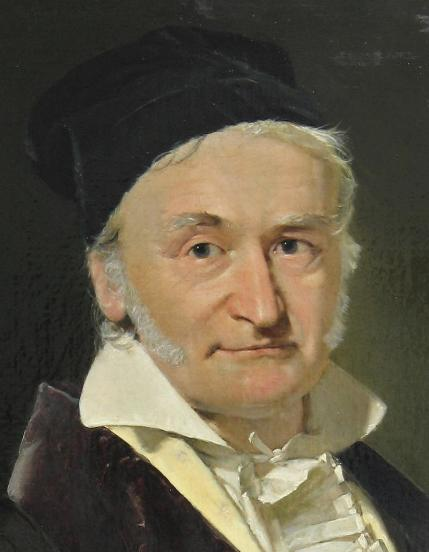
\includegraphics[width=0.4\textwidth]{gauss.png}
    \caption{Retrato de Gauss}
    \end{figure}
\end{columns}

 %*----------- notes
     \note[item]{Notes can help you to remember important information. Turn on the notes option.}
 \end{frame}
 %-
%----------------------------------------------------SLIDE------------------
 \begin{frame}[t]{References}
 %\frametitle{References}
%\begin{frame}{Reference}
    %\transboxin[duration=1,direction=30]

    % \begin{bibunit}[plain]
    % \cite{guangyi2018research}.
    % %\cite{kanakia2012}
    % %\cite{agostini2007}
    % %\cite{azuma1997survey}
    % \cite{Buss2005}
  
    % \putbib
    % \end{bibunit}
  
    %\bibliographystyle{IEEEtran}
    %\bibliographystyle{IEEEtranS}
    %\bibliographystyle{IEEEbib}
     \bibliographystyle{abntex2-alf}
    %\bibliographystyle{abntex2-num}
    %\bibliographystyle{abnt-alf}
    \bibliography{bibliography} 
    %\putbib

%*----------- notes
    %\note[item]{Notes can help you to remember important information. Turn on the notes option.}
\end{frame}
%
%-
%*----------- SLIDE-BACKUP ------------------------------------------------------
% \backupbegin
% %
% \begin{frame}{Backup}
%     Test
% %*----------- notes-------------------------------
% \note{Notes can help you to remember important information. Turn on the notes option.}
% \end{frame}
% %-
% \backupend
% %-
%*----------- QUESTIONS ---------------------------------------------------------
\begin{frame}[c,plain]
    \lastpage{
        \begin{center}   
            {\usebeamerfont{title} Questions?}\\[3ex] 
            %\hspace{1.5cm} 
            juliana.maria@fbter.org.br
        \end{center}
    }
    
    %*----------- notes---------------------------------
    \note[item]{Notes can help you to remember important information. Turn on the notes option.}
\end{frame}
%*-------------------------------------------------------------------------------
\end{document}